% =====================================================================
%  Figure 1 -- Architecture of the detect-ground-repair agent under study,
%  with the evaluation harness kept separate and RQ badges marking what each
%  research question probes.  ("Right Place, Wrong Fix")
%  Compile:  pdflatex fig1_architecture.tex
%  Edit:     PALETTE (colours), STYLES (box types), GRID (column x / row y).
% =====================================================================
\documentclass[tikz,border=4pt]{standalone}
\usepackage[T1]{fontenc}
\usepackage{mathptmx}
\usetikzlibrary{arrows.meta,shapes.geometric,positioning,backgrounds,calc,fit}

% ----------------------------- PALETTE -------------------------------
\definecolor{dataC}{HTML}{ECE8F4}  \definecolor{dataD}{HTML}{6B5B95} % data / inputs
\definecolor{slcC} {HTML}{FCE7CF}  \definecolor{slcD} {HTML}{C4651A} % slicing / static analysis
\definecolor{llmC} {HTML}{DCEAF8}  \definecolor{llmD} {HTML}{2E6DB4} % LLM components
\definecolor{evC}  {HTML}{F9DADF}  \definecolor{evD}  {HTML}{B23A48} % evaluation / oracle
\definecolor{laneC}{HTML}{F4F5F7}  \definecolor{laneD}{HTML}{CDD1D7} % frames
\definecolor{inkC} {HTML}{262626}  \definecolor{subC} {HTML}{555555} % text
\definecolor{rqC}  {HTML}{3A3F47}                                     % RQ badges

% ----------------------------- GRID ---------------------------------
\def\xIn{0}   \def\xGr{4.1}   \def\xAg{8.2}   \def\xOut{11.8}   \def\xEv{16.05}
\def\boxw{3.0cm}   \def\boxh{1.0cm}

\newcommand{\T}[1]{{\footnotesize\color{inkC}\textsc{#1}}}

\tikzset{
  >={Stealth[length=4.2pt,width=3.6pt]},
  box/.style 2 args={rectangle, rounded corners=2pt, draw=#2, fill=#1,
        line width=0.65pt, minimum width=\boxw, minimum height=\boxh,
        align=center, inner sep=2.5pt, font=\scriptsize, text=subC},
  data/.style  ={box={dataC}{dataD}},
  slicer/.style={box={slcC}{slcD}},
  llm/.style   ={box={llmC}{llmD}},
  eval/.style  ={box={evC}{evD}, line width=1.2pt},
  db/.style={cylinder, shape border rotate=90, aspect=0.17, draw=dataD,
        fill=dataC, line width=0.65pt, minimum width=2.85cm, minimum height=1.25cm,
        align=center, inner sep=1.5pt, font=\scriptsize, text=subC},
  flow/.style={->, line width=0.75pt, draw=inkC!75, rounded corners=2pt},
  ground/.style={->, line width=0.9pt, draw=llmD!80, rounded corners=2pt},
  fb/.style  ={->, line width=0.75pt, draw=llmD, dashed},
  truth/.style={->, line width=0.8pt, draw=evD, densely dotted},
  elab/.style={font=\scriptsize\itshape, text=subC, inner sep=1.2pt},
  rq/.style={rectangle, rounded corners=2.5pt, fill=rqC, text=white,
        font=\scriptsize\bfseries\sffamily, inner sep=1.6pt, minimum height=0.36cm},
  frame/.style={rounded corners=5pt, draw=laneD, fill=laneC, line width=0.6pt},
  hframe/.style={rounded corners=5pt, draw=evD!70, fill=evC!35, line width=0.9pt, dashed},
}

\begin{document}
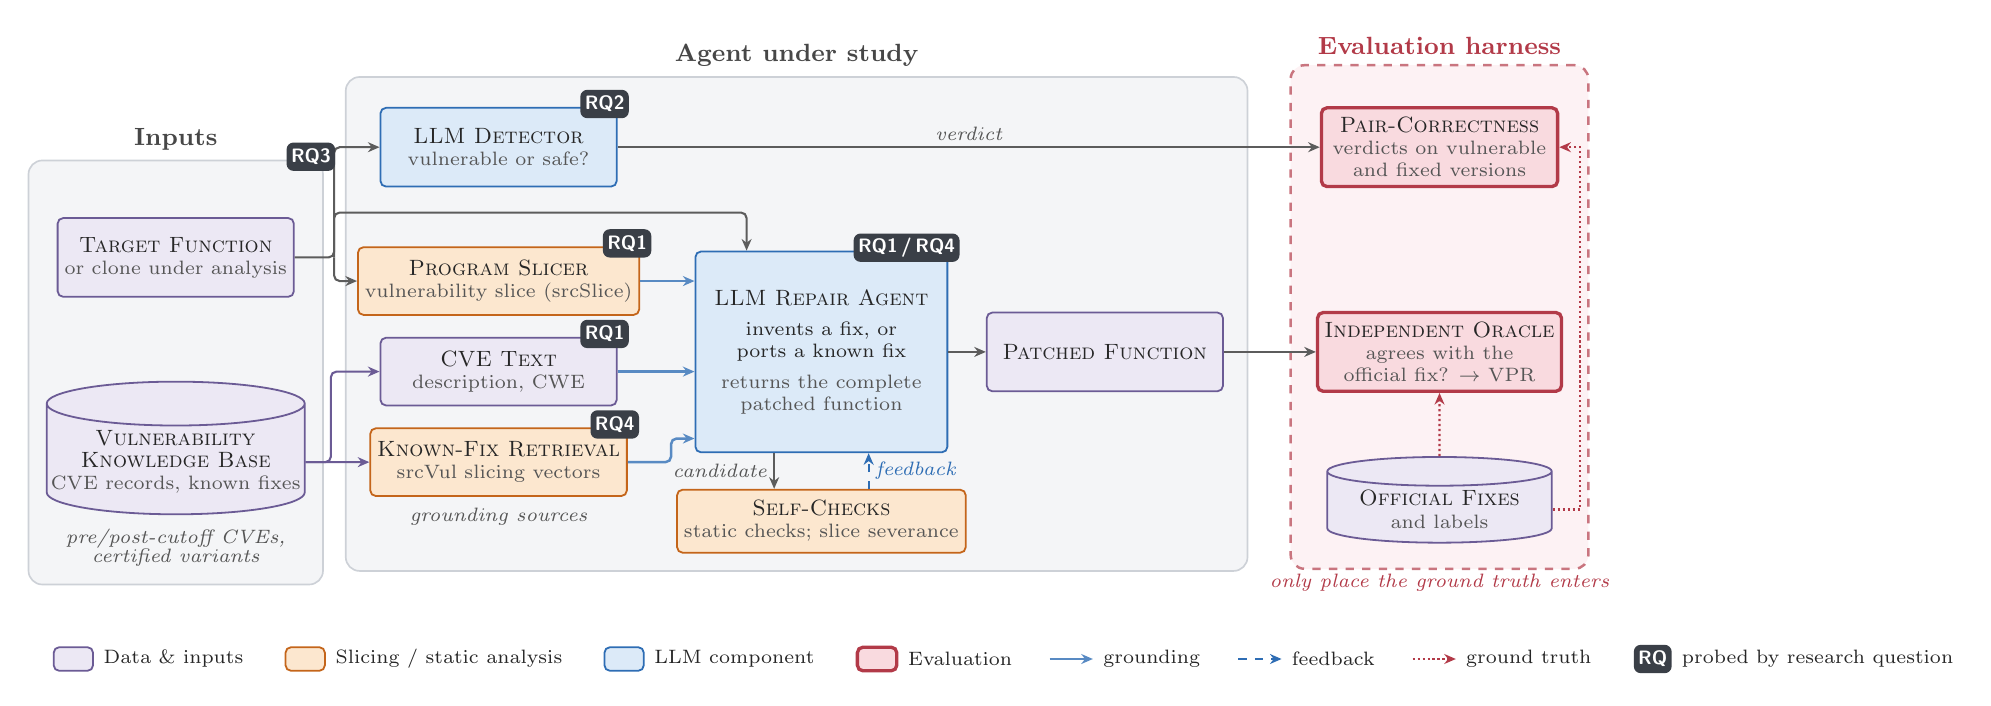
\begin{tikzpicture}

% =====================================================================
% INPUTS
% =====================================================================
\node[data] (target) at (\xIn,1.05)
      {\T{Target Function}\\or clone under analysis};
\node[db] (kb) at (\xIn,-1.55)
      {\T{Vulnerability}\\\T{Knowledge Base}\\CVE records, known fixes};

% =====================================================================
% DETECTION + GROUNDING SOURCES
% =====================================================================
\node[llm] (det) at (\xGr,2.45)
      {\T{LLM Detector}\\vulnerable or safe?};
\node[slicer, minimum height=0.86cm] (slicer) at (\xGr,0.75)
      {\T{Program Slicer}\\vulnerability slice (srcSlice)};
\node[data, minimum height=0.86cm] (cvetext) at (\xGr,-0.4)
      {\T{CVE Text}\\description, CWE};
\node[slicer, minimum height=0.86cm] (retr) at (\xGr,-1.55)
      {\T{Known-Fix Retrieval}\\srcVul slicing vectors};
\node[elab, anchor=north, align=center] (gsrc) at (\xGr,-2.08)
      {grounding sources};

% =====================================================================
% REPAIR AGENT
% =====================================================================
\node[llm, minimum width=3.2cm, minimum height=2.55cm] (agent) at (\xAg,-0.15)
      {\T{LLM Repair Agent}\\[3pt]
       \color{inkC}invents a fix, or\\\color{inkC}ports a known fix\\[3pt]
       returns the complete\\patched function};
\node[slicer, minimum width=3.2cm, minimum height=0.8cm] (checks) at (\xAg,-2.3)
      {\T{Self-Checks}\\static checks; slice severance};

\node[data] (patched) at (\xOut,-0.15) {\T{Patched Function}};

% =====================================================================
% EVALUATION HARNESS (separate; the only place the ground truth enters)
% =====================================================================
\node[eval] (pairc) at (\xEv,2.45) {\T{Pair-Correctness}\\verdicts on vulnerable\\and fixed versions};
\node[eval] (oracle) at (\xEv,-0.15) {\T{Independent Oracle}\\agrees with the\\official fix? $\to$ VPR};
\node[db, minimum height=1.05cm] (fixes) at (\xEv,-2.15) {\T{Official Fixes}\\and labels};

% =====================================================================
% FLOWS
% =====================================================================
% target into the system (one trunk: detector, slicer, agent)
\coordinate (tt) at ($(target.east)+(0.5,0)$);
\draw[flow] (target.east) -- (tt) |- (det.west);
\draw[flow] (tt) |- (slicer.west);
\draw[flow] (tt) |- (\xAg-0.95,1.62) -- ([xshift=-9.5mm]agent.north);
% knowledge base feeds CVE text and known fixes
\coordinate (kt) at ($(kb.east)+(0.32,0)$);
\draw[flow, draw=dataD] (kb.east) -- (kt) |- (cvetext.west);
\draw[flow, draw=dataD] (kb.east) -- (retr.west);
% grounding into the agent
\draw[ground] (slicer.east)  -- (slicer.east -| agent.west);
\draw[ground] (cvetext.east) -- (cvetext.east -| agent.west);
\draw[ground] (retr.east) -- ++(0.55,0) |- ([yshift=-11mm]agent.west);
% self-check loop
\draw[flow] ([xshift=-6mm]agent.south) -- node[elab, left=1pt]{candidate} ([xshift=-6mm]checks.north);
\draw[fb]   ([xshift=6mm]checks.north) -- node[elab, right=1pt, text=llmD]{feedback} ([xshift=6mm]agent.south);
% outputs to the harness
\draw[flow] (agent) -- (patched);
\draw[flow] (patched) -- (oracle);
\draw[flow] (det.east) -- node[elab, above=1pt, pos=0.5]{verdict} (pairc.west);
\draw[truth] (fixes) -- (oracle);
\draw[truth] (fixes.east) -- ++(0.35,0) |- (pairc.east);

% =====================================================================
% FRAMES (background) + RQ BADGES
% =====================================================================
\begin{scope}[on background layer]
  \node[frame, fit=(target)(kb), inner xsep=0.22cm, inner ysep=0.8cm, yshift=-0.08cm] (inframe) {};
  \node[frame, fit=(det)(retr)(agent)(checks)(patched)(gsrc), inner sep=0.3cm, yshift=0.08cm] (sysframe) {};
  \node[hframe, fit=(pairc)(oracle)(fixes), inner xsep=0.32cm, inner ysep=0.42cm, yshift=0.1cm] (harness) {};
\end{scope}
\node[font=\small\bfseries, text=inkC!85, anchor=south] at (inframe.north) {Inputs};
\node[font=\small\bfseries, text=inkC!85, anchor=south] at (sysframe.north) {Agent under study};
\node[font=\small\bfseries, text=evD, anchor=south] at (harness.north) {Evaluation harness};
\node[elab, anchor=north, align=center, text=evD] at (harness.south)
      {only place the ground truth enters};

% RQ badges
\node[rq, anchor=south east] at ([xshift=1.5mm,yshift=-1.5mm]inframe.north east) {RQ3};
\node[elab, anchor=north, align=center] at ([yshift=-1.2mm]kb.south)
      {pre/post-cutoff CVEs,\\[-1pt]certified variants};
\node[rq, anchor=south east] at ([xshift=1.5mm,yshift=-1.5mm]det.north east) {RQ2};
\node[rq, anchor=south east] at ([xshift=1.5mm,yshift=-1.5mm]slicer.north east) {RQ1};
\node[rq, anchor=south east] at ([xshift=1.5mm,yshift=-1.5mm]cvetext.north east) {RQ1};
\node[rq, anchor=south east] at ([xshift=1.5mm,yshift=-1.5mm]retr.north east) {RQ4};
\node[rq, anchor=south east] at ([xshift=1.5mm,yshift=-1.5mm]agent.north east) {RQ1\,/\,RQ4};

% =====================================================================
% LEGEND
% =====================================================================
\begin{scope}[shift={(-1.55,-4.05)}, every node/.style={font=\scriptsize, text=inkC}]
  \tikzset{key/.style={minimum width=0.5cm, minimum height=0.3cm, inner sep=0}}
  \node[data, key] (k1) at (0.25,0) {};
  \node[anchor=west] (t1) at (k1.east) {Data \& inputs};
  \node[slicer, key, right=0.4cm of t1] (k2) {};
  \node[anchor=west] (t2) at (k2.east) {Slicing / static analysis};
  \node[llm, key, right=0.4cm of t2] (k3) {};
  \node[anchor=west] (t3) at (k3.east) {LLM component};
  \node[eval, key, right=0.4cm of t3] (k4) {};
  \node[anchor=west] (t4) at (k4.east) {Evaluation};
  \draw[ground] ($(t4.east)+(0.35,0)$) -- ++(0.55,0) node[anchor=west] (t5) {grounding};
  \draw[fb]     ($(t5.east)+(0.35,0)$) -- ++(0.55,0) node[anchor=west] (t6) {feedback};
  \draw[truth]  ($(t6.east)+(0.35,0)$) -- ++(0.55,0) node[anchor=west] (t7) {ground truth};
  \node[rq, right=0.4cm of t7] (k8) {RQ};
  \node[anchor=west] at (k8.east) {probed by research question};
\end{scope}

\end{tikzpicture}
\end{document}
